\documentclass{article}
\usepackage{v-equation}

\geometry{
paperwidth=5in, 
paperheight=5in, 
top=10mm, 
bottom=10mm, 
left=10mm, 
right=10mm
}

\begin{document}
\begin{center}
Interference of light wave
\end{center}
\vspace*{\fill}
\begin{itemize}
\item[$\lambda$.] When two light waves of exactly equal frequency having constant phase difference with respect to time travelled in same direction and superimpose (overlap) with each other, then intensity of resultant wave does not remain uniform in space.
\end{itemize}

\begin{center}
\begin{tikzpicture}
[yscale=0.8]
	\def\Fn{sin(deg(\x))}
	\def\Fnn{-3*sin(deg(\x))}
	\def\Fnnn{2*sin(deg(\x))}
	\tzaxes(-0.5, -3.5)(7, 4){$t$}{$y$}
	\tzfn[dashed]\Fn[0:6.3]
	\tzfn[dashed]\Fnn[0:6.3]
	\tzfn\Fnnn[0:6.3]
	
	\tzvXpoint{Fn}(1.8,1)(C)
	\tzvXpoint{Fnn}(1.8,1)(B)
	\tzvXpoint{Fnnn}(1.8,1)(A)
	
	\tzlines+[<-](A)(1, 1)(1, 0){$y$}[r];
	\tzlines+[<-](B)(1, -1)(1, 0){$y_2$}[r];
	\tzlines+[<-](C)(1, 1)(1, 0){$y_1$}[r];
\end{tikzpicture}
\end{center}
\vspace*{\fill}

\pagebreak

\begin{center}
\begin{tikzpicture}
[yscale=0.8]
	\def\Fn{sin(deg(\x))}
	\def\Fnn{2*sin(deg(\x))}
	\def\Fnnn{3*sin(deg(\x))}
	\tzaxes(-0.5, -3.5)(7, 4){$t$}{$y$}
	\tzfn[dashed]\Fn[0:6.3]
	\tzfn[dashed]\Fnn[0:6.3]
	\tzfn\Fnnn[0:6.3]
	
	\tzvXpoint{Fn}(1.8,1)(C)
	\tzvXpoint{Fnn}(1.8,1)(B)
	\tzvXpoint{Fnnn}(1.8,1)(A)
	
	\tzlines+[<-](A)(1, 1)(1, 0){$y$}[r];
	\tzlines+[<-](B)(1, 1)(1, 0){$y_1$}[r];
	\tzlines+[<-](C)(1, 1)(1, 0){$y_2$}[r];
\end{tikzpicture}
\tikz\node at (0, 0) {\texttt{Constructive interference}};
\end{center}

\vspace*{\fill}
\begin{align*}
y = y_1 + y_2
\end{align*}
\vspace*{\fill}

\pagebreak
\begin{center}
\begin{tikzpicture}
[yscale=0.8]
	\def\Fn{2*sin(deg(\x))}
	\def\Fnn{-2*sin(deg(\x))}
	\def\Fnnn{0*sin(deg(\x))}
	\tzaxes(-0.5, -3.5)(7, 4){$t$}{$y$}
	\tzfn\Fn[0:6.3]
	\tzfn[dashed]\Fnn[0:6.3]
	\tzfn\Fnnn[0:6.3]
	
	\tzvXpoint{Fn}(1.8,1)(C)
	\tzvXpoint{Fnn}(1.8,1)(B)
	\tzvXpoint{Fnnn}(1.8,1)(A)
	
	\tzlines+[<-](A)(1, 1)(1, 0){$y$}[r];
	\tzlines+[<-](B)(1, 1)(1, 0){$y_2$}[r];
	\tzlines+[<-](C)(1, 1)(1, 0){$y_1$}[r];
\end{tikzpicture}
\tikz\node at (0, 0) {\texttt{Destructive interference}};
\end{center}
\vspace*{\fill}
\begin{align*}
y = y_1 + y_2
\end{align*}
\vspace*{\fill}
\pagebreak


\vspace*{\fill}
\begin{align*}
y &= (a+b)\sin\left(\omega t + \phi \right) &&- \texttt{superimposed wave}\\
y_1 &= a\sin\left(\omega t + \phi \right) &&- \texttt{first wave}\\
y_2 &= b\sin\left(\omega t + \phi \right) &&- \texttt{second wave}\\
\end{align*}

\vspace*{\fill}

\begin{center}
	\fbox{\qrcode[height=2cm]{https://drive.google.com/drive/folders/1FvC0YyNmmco0EVGxkNp4sY8lK47FySpp?usp=share_link}}
\end{center}

\end{document}
